We generalize the previous results by showing that over Poncelet 3-periodics in concentric, non-axis-aligned ellipse pairs, the power of the center with respect to either circumcircle or Euler's circle
is still invariant. This holds despite (i) their centers moving along non-axis aligned ellipses and (ii) their radii being variable.

The Cayley condition for the concentric version ($O_c=O$) of the pair in Figure~\ref{fig:n3-general-pos} which admits a 3-periodic family reduces to \cite{dragovic11}: 

%\[ a^2 \left(b^2-a_c^2\right)+\cos^2{\theta} c^2 (a_c^2-b_c^2)-2 a\,a_c\,b\,b_c-b^2 b_c^2 = 0\]

\[ a^2 b^2+\cos^2{\theta}~c^2 (a_c^2-b_c^2)-(a a_c+b b_c)^2 = 0\]

Note $\cos^2{\theta}$ can be expressed in terms of $a,b,a_c,b_c$:

%\[ \cos^2{\theta} =  \frac{2 a\,a_c\,b\,b_c+b^2 b_c^2-a^2 \left(b^2-a_c^2\right)}{c^2 (a_c^2-b_c^2)} \]

\[ \cos^2{\theta} =  \frac{(a a_c+b b_c)^2-a^2 b^2}{c^2 (a_c^2-b_c^2)} \]

As shown ion Figure~\ref{fig:cos-limits}, the feasible region of $a_c,b_c$ lies between to lines. Note that when $\theta=0$ the above reduces to:

\[ \frac{a_c}{a}+\frac{b_c}{b}=1 \]

\begin{figure}
    \centering
    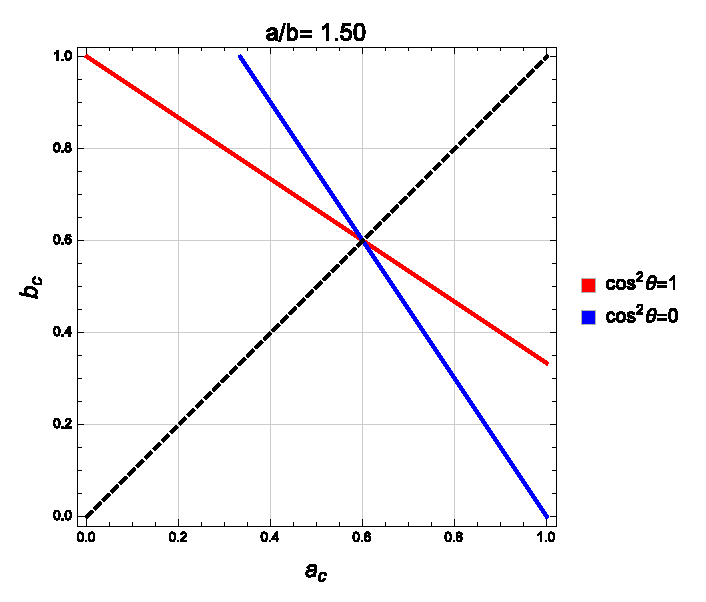
\includegraphics[width=.5\textwidth]{pics/0010_cayley_cos.eps}
    \caption{For a given choice of $a$ and $b$ (in the figure, $a=1.5$, $b=1$, the feasible region for $a_c$ and $b_c$ lies between the limit lines where $\cos^2(\theta)$ is 0 or 1, respectively.}
    \label{fig:cos-limits}
\end{figure}


 
Referring to Figure~\ref{fig:n3-tilted-circum-euler}, consider the family of 3-periodics interscribed between a concentric pair of ellipses $\E$ and $\E_c$, at an angle $\theta$ with each other.
Consider the pair of ellipses:

\begin{align*}
   \E&:  (b^2 + c^2)x^2  - 2 a c x y  + a^2 y^2 - b^2 a^2=0 \\
   \E_c&: \frac{x^2}{a_c^2}+\frac{y^2}{b_c^2}-1=0\\
\end{align*} 
where $-c^2a_c^2 + (ab + a b_c + a_c b)(ab - ab_c - a_c b)=0$.

\begin{proposition}
The locus of $X_3$ and $X_5$ are ellipses $\E_3$, and $\E_5$  which are concentric with the pair. Furthermore, $\E_3$ is axis-aligned with $\E_c$ and its aspect ratio is equal to $b_c/a_c$. $\E_3$ is given by:

\begin{align*}
%\E_3:&-4\,{b}^{2}a_c^{2} \left( a_c^{2}{x}^{2}+b_c^{2}{y}^{2} \right) \\
%&+b_c^{2} \left(  \left( a_c^{2}+{b}^{2}-{
%b_c}^{2} \right) a+2\,a_c\, \left( a_c-b_c
 %\right) b \right)  \left(  \left( a_c^{2}+{b}^{2}-b_c^{
%2} \right) a-2\,a_c\, \left( a_c+b_c \right) b \right) =0
%
\E_3:&\; 4\,{b}^{2}a_c^{2} \left( a_c^{2}{x}^{2}+b_c^{2}{y}^{2} \right)  
 -b_c^{2} \left(  \left( a_c^{2}-
b_c^{2} +{b}^{2}\right)^2 a^2 -4\,a_c^2b^2\, \left( a_c-b_c
 \right)^2   \right)    =0
\end{align*}
\label{prop:loci-x3-x5}

\noindent The axes of $\E_5$ are given by

\begin{align*}
    a_5&=\frac{\sqrt{2} (a a_c^2 b_c + a b^2 b_c - a b_c^3 - 2 a_c^3 b - 2 a_c b b_c^2)}{8 a_c^2 b}\\
    b_5&=\frac{\sqrt{2} (a a_c^2 - 4 a_c b b_c + a (b^2 - b_c^2))}{8 b a_c}
\end{align*} 
\end{proposition}

\begin{observation}
For the special case where the pair is axis-aligned $(\theta=0)$ the expression for $\E_5$ is tractable, and given by:

\[\E_5: \; \frac{ 16 a^4x^2}{(a^3 - 3 a^2  a_c + a b^2 -  a_c b^2)^2}+\frac{16 b^2 a^2y^2}{ (a^2  a_c - 2 a b^2 + 3  a_c b^2)^2}-1=0\]
\end{observation}

Now we are in a position to prove our first main result:

\begin{theorem}
The power of the common center $O$ is invariant with respect to either the circumcircle or the Euler circle and given by:

\begin{align*}
    \P_3  &=-\frac{a b_c}{b a_c}\left(b^2 + a_c^2 - b_c^2 \right)- (a_c^2 - b_c^2) \\
    \P_5&= -\frac{a b_c}{2 b a_c}\left(b^2 + a_c^2 - b_c^2 \right)+b_c^{2}
%    \P_5  &=-\frac{(aa_c^2 + ab^2 - ab_c^2 - 2a_cb_cb)b_c}{2a_cb }  
\end{align*}

\label{thm:power-concentric-unaligned}
\end{theorem}

\begin{proof}
We write explicit parametrized expressions for the vertices of 3-periodics in a generic concentric pair. We write out explicit expressions for circumcenter, Euler center, and circumradius and finally the power of the center with respect to these. Via a process of laborious manual CAS-based simplification, we arrive at the result.
\end{proof}

\noindent Notice that $2\P_5-\P_3=a_c^2+b_c^2$.

\begin{observation}
When the ellipses are concentric and axis-aligned, Theorem~\ref{thm:power-concentric-unaligned} reduces to:

\[ \P_3  = -\frac{a_c}{a}c^2 - b^2,\;\;\;\P_5 =-\frac{{a_c} (a-{a_c}) \left(a^2+b^2\right)}{2 a^2}\]
\end{observation}

\begin{figure}
    \centering
    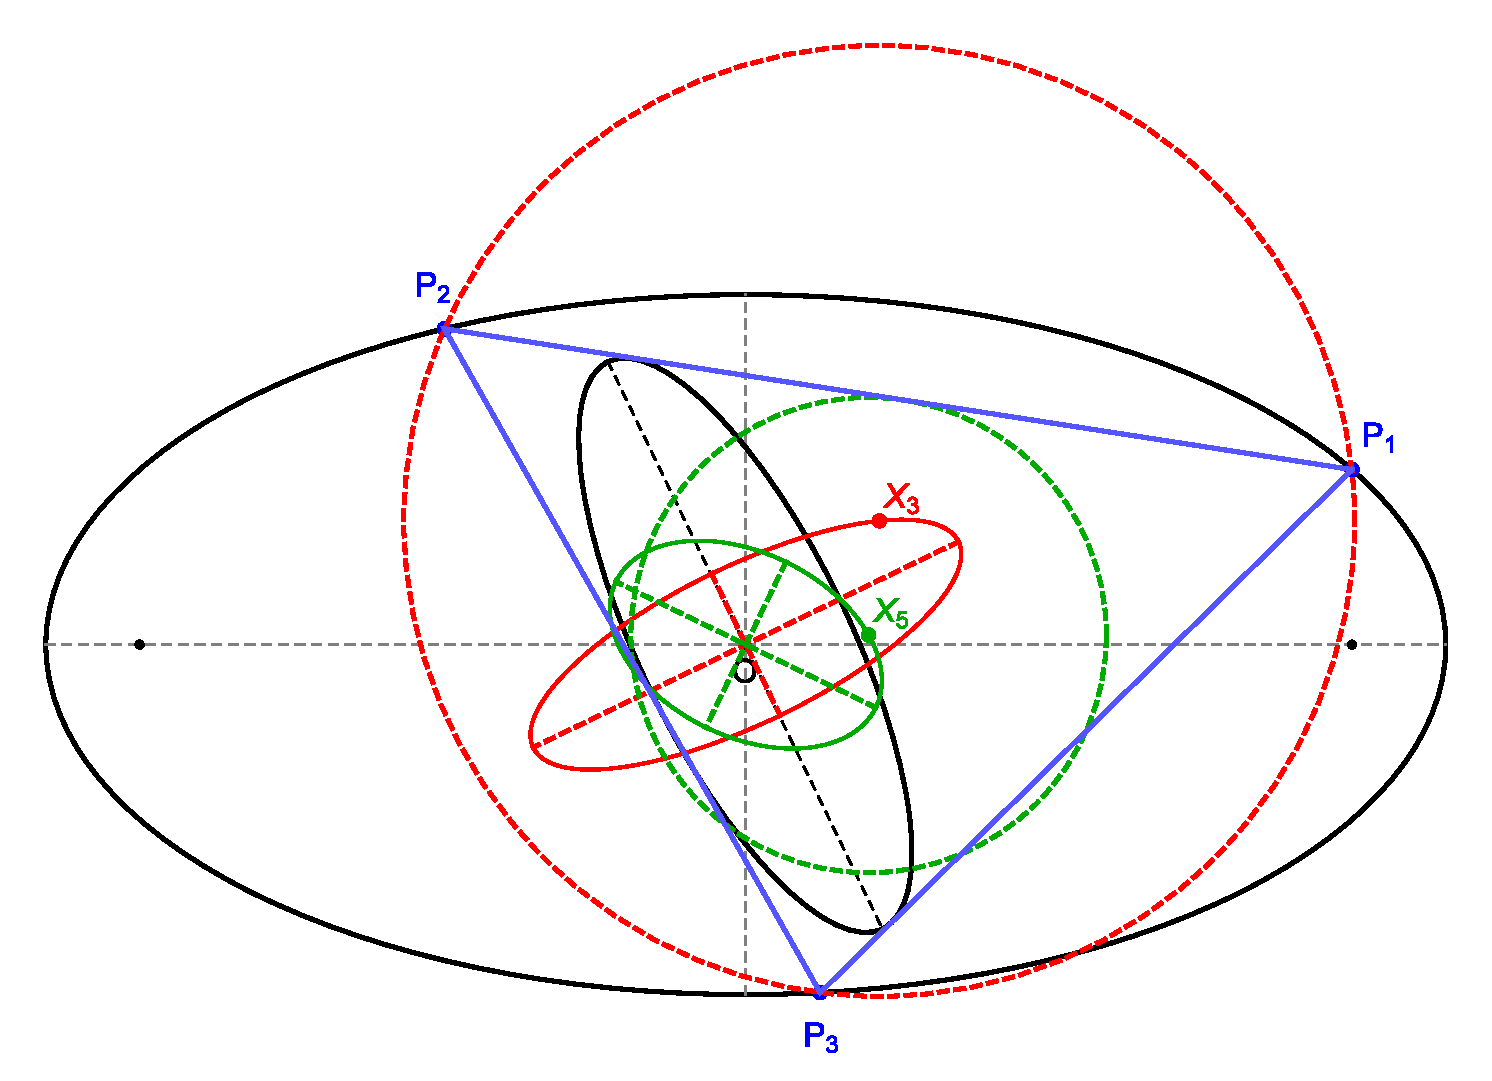
\includegraphics[width=.7\textwidth]{pics/0030_n3_circum_euler.eps}
    \caption{Over the family of 3-periodics (blue) interscribed in a pair of concentric, unaligned ellipses, the locus of $X_3$ and $X_5$ are also ellipses (red and green) which are concentric with the original pair. Furthermore, the locus of $X_3$ is axis-aligned with the inner ellipse. Remarkably, the power of the common center $O$ with respect to either the circumcircle (dashed red) or Euler's circle (dashed green) is invariant.}
    \label{fig:n3-tilted-circum-euler}
\end{figure}

Referring to Figure~\ref{fig:concentric-xns}, consider the concentric, unaligned pair of ellipses $\E$ and $\E_c$ given by:

\[ 
    \E:\,\frac{x^2}{a^2}+\frac{y^2}{b^2}-1=0,\;\;\;
    \E_c:\,(b_c^2 + \zeta^2)x^2  - 2 a_c \zeta x y  + a_c^2 y^2 - b_c^2 a_c^2=0\\
\]

where $\zeta$ is defined relative to $\theta$ as follows:

\[\tan{2\theta}=\frac{2 a\zeta}{c^2 - \zeta^2}\]

Furthermore the Cayley condition reduces to:

\[a^2 \zeta^2 - (a b + a b_c + a_c b)(a b - a b_c - a_c b)=0\]
%\[a_1^2b^2 + 2a_1b_1ab + b_1^2a^2 - a^2b^2 + c_1^2a^2=0\]

\begin{figure}
     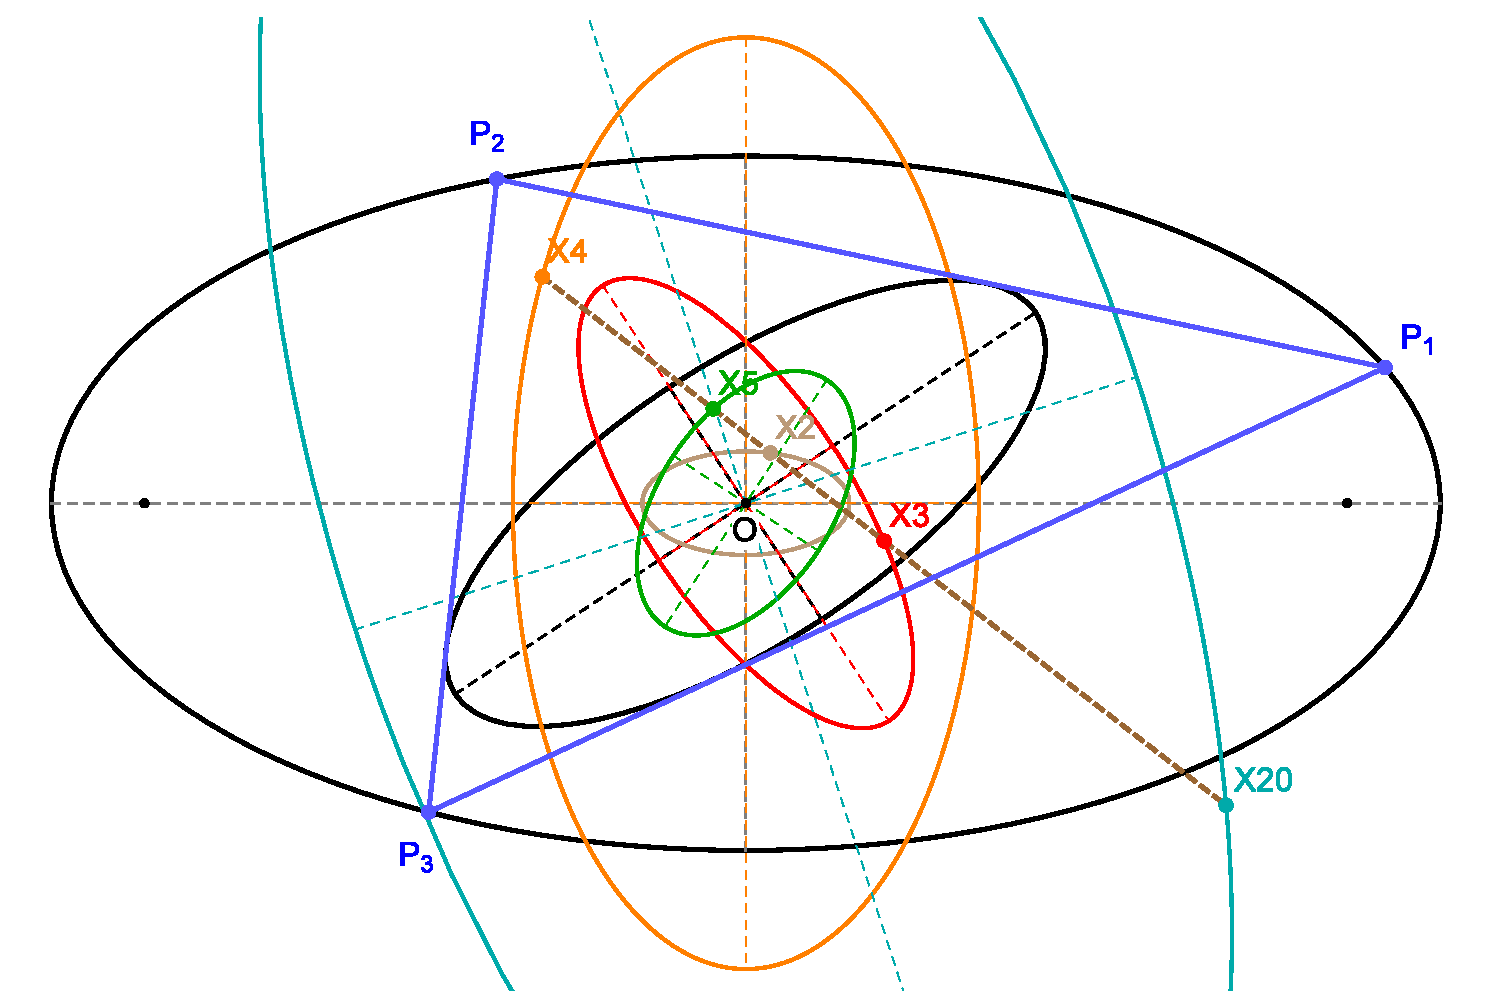
\includegraphics[width=\textwidth]{pics/0080_n3_concentric_conics.eps}
     \caption{In the concentric-tilted pair (black ellipses), the loci of $X_k$, $k=2,3,4,5,20$ are ellipses. The Euler line (dashed brown) connect said centers. \href{https://youtu.be/hpb7ZgKWjUY}{Video}}
     \label{fig:concentric-xns}
 \end{figure}

\subsection*{Generalizing invariant center power}

Recall a pencil of coaxial circles has collinear centers and identical limiting points \cite[Coaxal Circles]{mw}.

The radical axis of the pencil of circles containing the circumcircle and Euler's circle is known as the ``orthic axis'' and it is perpendicular to the Euler line\footnote{The Euler line and the orthic axis intersect at $X_{468}$.} \cite[Orthic Axis]{mw}.

\begin{proposition}
Over Poncelet 3-periodics in a concentric pair (axis-aligned or not) with center at $O$, let $\C$ be a circle coaxial with both circumcenter and Euler's circle, such that its center $X$ is a fixed affine combination of $X_3$ and $X_5$. The power of $O$ with respect $\C$ is invariant.
\label{prop:coaxial}
\end{proposition}

\begin{proof}

Let $\P(M,\C_0)$ denote the power of point $M\in\R^2$ with respect to a circle $\C_0$.

Let $\C_3$ (resp. $\C_5$) denote the circumcircle (resp. Euler's circle) of 3-periodics in a concentric pair centered on $O$. Let $X_3$ and $R$ (resp. $X_5$ and $r_5=R/2$) denote the center and radius of $\C_3$ (resp. $\C_5$). Let $r_X$ denote the radius of $\C$, a circle coaxial with $\C_3$ and $\C_5$, centered at $X$.

Let $t$ be a fixed real number, so that $X=t X_3+(1-t)X_5$ is a fixed affine combination $X_3$ and $X_5$. By Theorem \ref{thm:power-concentric-unaligned}, $\P(O,\C_3)$ and $\P(O,\C_5)$ are both invariant over 3-periodics in a concentric pair.

In the remainder of this proof we show that in fact:

\[ \P(O,\C)=t\P(O,\C_3)+(1-t)\P(O,\C_5)\]
which entails our claim.

Take a single 3-periodic in the aforementioned family. Since both statements $X=t X_3+(1-t)X_5$ and $\P(O,\C)=t\P(O,\C_3)+(1-t)\P(O,\C_5)$ are invariant under rotations and translations of the plane, assume without loss of generality that the line through $X_3$, $X_5$, and $X$ (Euler line) is the x-axis and that the common radical axis of $\C_3$, $\C_5$, and $\C$ (orthic axis) is the y-axis. Let $T$ be the origin of this coordinate system ($X_{468}$ of the 3-periodic triangle).

Let $X_3=(x_3,0)$ and $X_5=(x_5,0)$ so that $X=(t x_3+(1-t)x_5,0)$. Also, let $O=(u,v)$ in this new coordinate system. For an arbitrary point $P=(x_P,0)$ on the line through $X_3$, $X_5$, we denote by $\C_P$ the circle centered at $P$ that is coaxial with $\C_3$ and $\C_5$, and its radius by $r_P$.

Since $T$ is on the radical axis of the pencil of coaxial circles of $\C_3$ and $\C_5$, its power with respect to any of the circles in this pencil is the same, so we denote it as $\P_T$. See that 
\begin{gather*}
    \P(O,\C_P)=|O P|^2-{r_P}^2= (u-x_P)^2+v^2-{r_P}^2=\\
    =(u^2+v^2)+(x_P^2-r_P^2)-2 u x_P= \|O\|^2+\P_T-2 u x_P
\end{gather*}

Using this identity with $P=X_3$, $P=X_5$, and $P=X$, we get
\begin{gather*}
    t\P(O,\C_3)+(1-t)\P(O,\C_5)=\\
    =t(\|O\|^2+\P_T-2 u x_3)+(1-t)(\|O\|^2+\P_T-2 u x_5)=\\
    \|O\|^2+\P_T-2 u (t x_3+(1-t)x_5)=\P(O,\C)
\end{gather*}
\end{proof}

An illustration to Proposition \ref{prop:coaxial} is provided by a well-known group of circles coaxial with the circumcircle and the Euler circle, listed in  Table~\ref{tab:coaxal-circles} and shown in Figure~\ref{fig:coaxal-power}.

\begin{table}
    \centering
    \begin{tabular}{|r|c|c|}
    \hline
    name & center & squared radius \\ \hline
        Circumcircle & $X_5$ & $R^2$ \\
        Euler's circle & $X_3$ & $R^2/4$ \\
        Steiner orthoptic circle & $X_2$ & ${\sum{s_i}^2}/18$ \\
        Orthocentroidal & $X_{381}$ & $R^2-\sum{s_i}^2/9$ \\
        Polar$^\dagger$ circle & $X_4$ & $4 R^2-(\sum{s_i}^2)/2$ \\
        Tangential$^\ddagger$ circle& $X_{26}$ & ${R^2}/({16|\prod{\cos\theta_i}|^2})$ \\
        \hline
    \end{tabular}
    \caption{Six coaxial circles with centers on the Euler line \cite[Coaxal System]{mw}. $^\dagger$The squared radius of the polar circle is positive (resp. negative) for obtuse (resp. acute) triangles. Its signed squared radius is used when computing circle power. $^\ddagger$The tangential circle is the only in the list whose center is not a fixed linear combination of $X_3$ and $X_5$.}
    \label{tab:coaxal-circles}
\end{table}

\begin{observation}
The power of the center wrt to the coaxial circles listed on Table~\ref{tab:coaxal-circles} is invariant, with the exception of the tangential circle, since the latter's center is not a fixed linear combination of $X_3$ and $X_5$.
\label{obs:coaxial}
\end{observation}

\begin{figure}
    \centering
    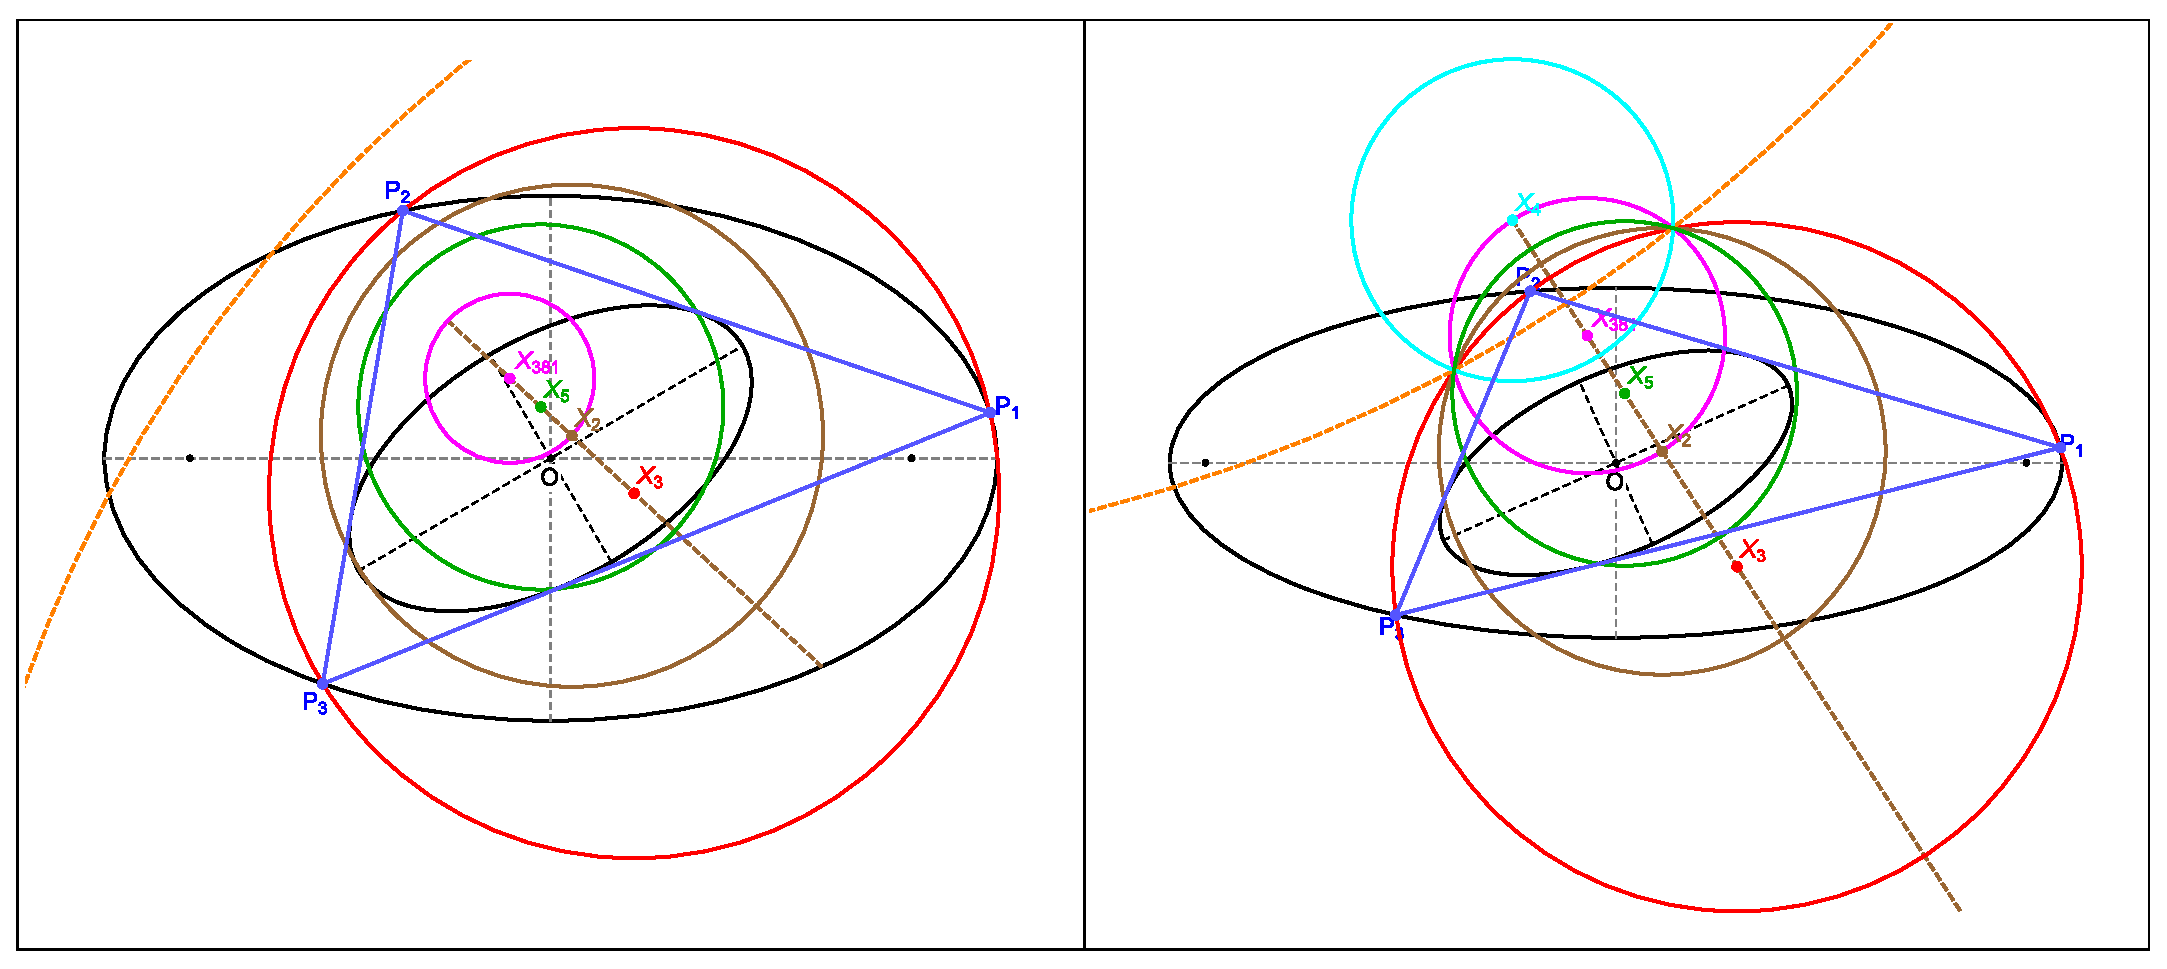
\includegraphics[width=\textwidth]{pics/0155_coaxal_power_both_sides.eps}
    \caption{\textbf{Top:} An acute 3-periodic (blue) is shown in a concentric, unaligned pair. The power of the center is invariant with respect to the following set of coaxial circles whose centers lie at linear combinations of $X_3$ and $X_5$: circumcircle (red), Euler's (green), Steiner's inellipse orthoptic (brown), orthocentroidal (magenta), centered on $X_k$, $k=$3,5,2,381, respectively. The power of the center wrt to the also coaxial tangential circle (dashed orange) is variable as expected, since its center $X_{26}$ is not a fixed linear combination of $X_3$ and $X_5$. \textbf{Bottom:} an obtuse 3-periodic (blue) is shown in a concentric, unaligned pair. All coaxial circles now intersect at two common points. The polar circle (cyan) is now defined, centered on $X_4$. The power of the center wrt to all circles shown (except for the tangential, dashed orange) is constant.}
    \label{fig:coaxal-power}
\end{figure}

\begin{proposition}
Over 3-periodics in the concentric, non-axis aligned ellipse pair, the loci of $X_2$ and $X_4$ are ellipses concentric and axis-aligned with the outer one, given by:

\begin{align*}
X_2:& \; 9b^2x^2 + 9a^2y^2 + ab(4a_1b_1 - ab)=0\\
X_4:&\; (a^4 - b^4)a_1^2 - 2ab(a^2 + b^2)a_1b_1 + a^2b^4 - a^2(a^2x^2 + b^2y^2)=0
\end{align*}
\end{proposition}

\subsection*{Generalizing elliptic loci}

The following is a special case of Theorem~\ref{thm:ellipse-locus}, whose proof appears in Section~\ref{sec:nonconcentric-tilted}:

\begin{proposition}
If a triangle center $\X_\gamma=(1-\gamma) X_2+ \gamma X_3$ is a fixed affine combination of $X_2$ and $X_3$ for some $\gamma\in\R$, its locus over 3-periodics in the concentric, non-axis-aligned ellipse pair will be an ellipse.
\label{prop:concentric}
\end{proposition}

There are 226 triangle centers on \cite{etc} which are fixed linear combinations of $X_2$ and $X_3$; see Observation~\ref{obs:affine-euler-line}. Experimentally, these are also the only ones which trace out ellipses.

Consider the converse of Proposition~\ref{prop:concentric}. If for some concentric, non-axis aligned pair some triangle center $\X$ has an elliptic locus, can it be affirmed that $\X$ is a fixed linear combination of $X_2$ and $X_3$? Consider the case of the Steiner point $X_{99}$. This point is known to lie on the Euler line, circumcircle, and Steiner circumellipse, although it is not a fixed linear combination of $X_2$ and $X_3$ \cite{etc}. Still, over (i) the homothetic family, and (ii) the family with circumcircle, its locus is (i) the outer (Steiner) ellipse, and (ii) the outer circle. However, over the confocal family, the locus of $X_{99}$ is non-elliptic.

Based on experimental evidence, in Conjecture~\ref{conj:concentric} (Section~\ref{sec:open-questions}) we state a converse to Proposition~\ref{prop:concentric}.

